\documentclass[a4paper,12pt]{article}

% ==============================================================================
% PACKAGES & CONFIGURATION
% ==============================================================================
\usepackage[utf8]{vietnam}
\usepackage[a4paper,top=2.5cm,bottom=2.5cm,left=3cm,right=2cm]{geometry}
\usepackage{graphicx}
\graphicspath{{./}{bao_cao/}{img/}{bao_cao/img/}}
\usepackage{amsmath,amssymb}
\usepackage{xcolor}
\usepackage{colortbl}
\usepackage{array}
\usepackage{caption}
\usepackage{booktabs}
\usepackage{tabularx}
\usepackage{float}
\usepackage{listings}
\usepackage{fancyhdr}
\usepackage{titlesec}
\usepackage{tikz}
\usepackage{tocloft}
\usepackage[numbib, nottoc]{tocbibind}
\usepackage[unicode, hidelinks]{hyperref}
\usetikzlibrary{shapes.geometric, arrows, positioning, fit, calc}

% Header and Footer setup
\setlength{\headheight}{18pt}
\setlength{\headsep}{22pt}
\pagestyle{fancy}
\fancyhf{}
\fancyhead[L]{\footnotesize\textit{LAN Chat \& File Sharing}}
\fancyhead[R]{\footnotesize\textit{Đồ án Mạng Máy Tính -- HCMUS}}
\fancyfoot[C]{\thepage}
\renewcommand{\headrulewidth}{0.4pt}
\renewcommand{\footrulewidth}{0.4pt}
\captionsetup[table]{justification=centering, singlelinecheck=false, labelfont={bf,color=blue!80!black}, textfont={bf,color=blue!80!black}, skip=6pt}

\newcommand{\code}[1]{\texttt{#1}}

% Code listing styling
\definecolor{codegreen}{rgb}{0,0.6,0}
\definecolor{codegray}{rgb}{0.5,0.5,0.5}
\definecolor{codepurple}{rgb}{0.58,0,0.82}
\definecolor{backcolour}{rgb}{0.96,0.96,0.96}

\lstdefinestyle{mystyle}{
	backgroundcolor=\color{backcolour},   
	commentstyle=\color{codegreen},
	keywordstyle=\color{magenta},
	numberstyle=\tiny\color{codegray},
	stringstyle=\color{codepurple},
	basicstyle=\ttfamily\footnotesize,
	breakatwhitespace=false,         
	breaklines=true,                 
	captionpos=b,                    
	keepspaces=true,                 
	numbers=left,                    
	numbersep=5pt,                  
	showspaces=false,                
	showstringspaces=false,
	showtabs=false,                  
	tabsize=2
}
\lstset{style=mystyle}

% Section formatting
\titleformat{\section}{\normalfont\Large\bfseries\color{blue!80!black}}{\thesection.}{1em}{}
\titleformat{\subsection}{\normalfont\large\bfseries\color{black}}{\thesubsection.}{1em}{}
\titleformat{\subsubsection}{\normalfont\normalsize\bfseries}{\thesubsubsection.}{1em}{}

% ------------------------------------------------------------------------------
% TÙY CHỈNH MỤC LỤC, DANH SÁCH HÌNH, DANH SÁCH BẢNG
% ------------------------------------------------------------------------------
\renewcommand{\cfttoctitlefont}{\normalfont\LARGE\bfseries\color{blue!80!black}}
\renewcommand{\cftloftitlefont}{\normalfont\LARGE\bfseries\color{blue!80!black}}
\renewcommand{\cftlottitlefont}{\normalfont\LARGE\bfseries\color{blue!80!black}}

\AtBeginDocument{
	\renewcommand{\contentsname}{MỤC LỤC}
	\renewcommand{\listfigurename}{DANH SÁCH HÌNH}
	\renewcommand{\listtablename}{DANH SÁCH BẢNG}
	\renewcommand{\refname}{Tài liệu tham khảo}
}

\renewcommand{\cftsecaftersnum}{.}
\renewcommand{\cftsubsecaftersnum}{.}
\renewcommand{\cftsubsubsecaftersnum}{.}
\setlength{\cftsecnumwidth}{2em}
\setlength{\cftsubsecnumwidth}{2.8em}
\setlength{\cftsubsubsecnumwidth}{3.5em}

\renewcommand{\cftfigpresnum}{Hình }
\renewcommand{\cftfigaftersnum}{.}
\setlength{\cftfignumwidth}{4.5em}

\renewcommand{\cfttabpresnum}{Bảng }
\renewcommand{\cfttabaftersnum}{.}
\setlength{\cfttabnumwidth}{4.5em}

% TikZ styles
\tikzstyle{block} = [rectangle, draw=blue!75!black, fill=blue!5, thick, rounded corners=4pt, text centered, minimum height=2.2em, inner sep=6pt]
\tikzstyle{arrow} = [thick, ->, >=stealth]
\tikzstyle{darrow} = [thick, <->, >=stealth]

% ==============================================================================
% DOCUMENT BEGIN
% ==============================================================================
\begin{document}
	
	% ------------------------------------------------------------------------------
	% COVER PAGE
	% ------------------------------------------------------------------------------
	\newgeometry{left=2.2cm, right=2.2cm, top=2.4cm, bottom=2.4cm}
	\begin{titlepage}
		\begin{tikzpicture}[remember picture, overlay]
			\draw[line width=1.5pt] 
			([xshift=1.8cm, yshift=-1.8cm]current page.north west) 
			rectangle 
			([xshift=-1.8cm, yshift=1.8cm]current page.south east);
			
			\draw[line width=0.5pt] 
			([xshift=1.92cm, yshift=-1.92cm]current page.north west) 
			rectangle 
			([xshift=-1.92cm, yshift=1.92cm]current page.south east);
		\end{tikzpicture}
		
		\centering
		\vspace*{0.3cm}
		{\Large \textbf{ĐẠI HỌC QUỐC GIA THÀNH PHỐ HỒ CHÍ MINH}}\\[0.15cm]
		{\Large \textbf{TRƯỜNG ĐẠI HỌC KHOA HỌC TỰ NHIÊN}}\\[0.15cm]
		{\large KHOA CÔNG NGHỆ THÔNG TIN}\\
		{\large MÔN MẠNG MÁY TÍNH}\\[0.6cm]
		
		\IfFileExists{HCMUS.png}{
\includegraphics[width=0.45\textwidth]{HCMUS.png}}{\vspace{3cm}}\\[0.7cm]
		
		{\large \bfseries BÁO CÁO ĐỒ ÁN THỰC HÀNH}\\[0.25cm]
		{\fontsize{20}{24}\selectfont \textbf{ỨNG DỤNG LAN CHAT \& FILE SHARING}}\\[0.8cm]
		
		\renewcommand{\arraystretch}{1.35} 
		\begin{tabular}{r l l}
			\textbf{Giảng viên hướng dẫn:} & ThS. Chung Thùy Linh & \\
			& ThS. Huỳnh Thụy Bảo Trân & \\[0.3cm]
			\textbf{Sinh viên thực hiện:}   & Nguyễn Đăng Huỳnh Nhân & -- \textbf{MSSV:} 25127221 \\
			& Đào Vạn Đức            & -- \textbf{MSSV:} 25127036 \\
			& Nguyễn Minh Huân       & -- \textbf{MSSV:} 25127050 \\[0.3cm]
			\textbf{Lớp:}                  & 25C04 &
		\end{tabular}
		
		\vfill
		{\large \textbf{Thành phố Hồ Chí Minh, Năm 2026}}
		\vspace*{0.2cm}
	\end{titlepage}
	\restoregeometry
	
	% ------------------------------------------------------------------------------
	% TABLE OF CONTENTS
	% ------------------------------------------------------------------------------
	\clearpage
	\pagenumbering{roman}
	\tableofcontents
	\clearpage
	\phantomsection
	\listoffigures
	\phantomsection
	\listoftables
	\clearpage
	\pagenumbering{arabic}
	
	% ------------------------------------------------------------------------------
	% SECTION 1: GIỚI THIỆU
	% ------------------------------------------------------------------------------
	\section{Giới thiệu}
	
	\subsection{Mục tiêu}
	Đề tài xây dựng một ứng dụng dòng lệnh (CLI) cho phép các máy trong cùng mạng LAN:
	\begin{itemize}
		\item tự tìm thấy nhau mà không cần máy chủ trung gian (mô hình ngang hàng, peer-to-peer),
		\item trò chuyện với nhiều người cùng lúc, có đếm tin chưa đọc và xem lại lịch sử,
		\item gửi và nhận tập tin, có thanh tiến trình.
	\end{itemize}
	Chương trình viết bằng Python 3.10 trở lên, chỉ dùng thư viện chuẩn (\code{socket}, \code{threading}, \code{struct}, \code{json}). Thư viện \code{prompt\_toolkit} là tùy chọn, dùng để hiển thị dòng nhập và thanh tiến trình đẹp hơn.
	
	\subsection{Các lệnh người dùng}
	
	\begin{table}[H]
		\centering
		\small
		\renewcommand{\arraystretch}{1.35}
		\begin{tabularx}{\textwidth}{|>{\raggedright\arraybackslash}p{4.8cm}|X|}
			\hline
			\rowcolor{blue!12}
			\textcolor{blue!80!black}{\textbf{Lệnh}} & \textcolor{blue!80!black}{\textbf{Ý nghĩa}} \\
			\hline
			\code{/list} & Xem danh sách bạn bè đang online, trạng thái kết nối và số tin chưa đọc \\
			\hline
			\code{/chat <tên|số|port|ip:port>} & Mở hoặc chuyển sang phòng chat với một người \\
			\hline
			\code{/msg <tên|port> <nội dung>} & Gửi một tin nhanh mà không mở phòng chat \\
			\hline
			\code{/send <đường dẫn>} & Gửi tập tin cho người đang chat \\
			\hline
			\code{/leave} & Rời phòng chat hiện tại (kết nối vẫn giữ, tin đến sẽ là chưa đọc) \\
			\hline
			\code{/status online|away} & Đổi trạng thái hiển thị \\
			\hline
			\code{/history [tên]} & Xem lịch sử tin nhắn \\
			\hline
			\code{/help}, \code{/quit} & Xem trợ giúp, thoát chương trình \\
			\hline
		\end{tabularx}
		\caption{Danh sách các lệnh người dùng hỗ trợ}
		\label{tab:user_commands}
	\end{table}
	
	\subsection{Cách chạy}
	\begin{lstlisting}[language=bash, caption={Lệnh cài đặt thư viện tùy chọn và khởi chạy ứng dụng}]
		python -m pip install -r requirements.txt
		python main.py --name A --tcp-port 5001
		python main.py --name B --tcp-port 5002
	\end{lstlisting}
	Muốn thử nhiều tiến trình trên cùng một máy, thêm tham số \code{-\/-broadcast-ip 127.255.255.255}.
	
	% ------------------------------------------------------------------------------
	% SECTION 2: KIẾN TRÚC
	% ------------------------------------------------------------------------------
	\section{Kiến trúc}
	
	\subsection{Mô hình phân lớp}
	Mã nguồn chia thành năm lớp. Lớp trên gọi lớp dưới, không gọi ngược lại (Hình~\ref{fig:architecture}).
	
	\begin{figure}[H]
		\centering
		\begin{tikzpicture}[
			box/.style={draw, rounded corners=2pt, align=center, minimum height=1.1cm, inner sep=4pt},
			arr/.style={->, >=stealth}]
			\node[box, minimum width=11.4cm] (ui) at (0,0) {\textbf{Giao diện}\\ \small cli.py, ui/console.py, ui/input\_handler.py, ui/progress\_display.py};
			\node[box, minimum width=11.4cm] (app) at (0,-2) {\textbf{Điều phối}\\ \small main.py, app.py (lớp \code{ChatApp})};
			\node[box, minimum width=5.3cm] (core) at (-2.95,-4.3) {\textbf{Lõi nghiệp vụ}\\ \small PeerManager, ChatManager,\\ MessageManager,\\ StatusManager};
			\node[box, minimum width=5.3cm] (tr) at (2.95,-4.3) {\textbf{Truyền tập tin}\\ \small TransferManager, FileSender,\\ FileReceiver,\\ TransferProgress};
			\node[box, minimum width=11.4cm] (net) at (0,-6.6) {\textbf{Mạng}\\ \small network/protocol.py, tcp\_server.py, tcp\_client.py,\\ udp\_broadcast.py, udp\_listener.py};
			\draw[arr] (ui) -- (app);
			\draw[arr] (app.south -| core.north) -- (core.north);
			\draw[arr] (app.south -| tr.north) -- (tr.north);
			\draw[arr] (tr.south) -- (tr.south |- net.north);
			\draw[arr] (app.east) -- ++(0.5,0) |- (net.east);
		\end{tikzpicture}
		\caption{Các lớp của chương trình (file \code{config.py} chứa tham số dùng chung cho mọi lớp)}
		\label{fig:architecture}
	\end{figure}
	
	\begin{table}[H]
		\centering
		\small
		\renewcommand{\arraystretch}{1.35}
		\begin{tabularx}{\textwidth}{|>{\raggedright\arraybackslash}p{2.6cm}|>{\raggedright\arraybackslash}p{4.3cm}|X|}
			\hline
			\rowcolor{blue!12}
			\textcolor{blue!80!black}{\textbf{Lớp}} & \textcolor{blue!80!black}{\textbf{Thành phần}} & \textcolor{blue!80!black}{\textbf{Vai trò}} \\
			\hline
			Giao diện & \code{CLI}, \code{Console}, \code{InputHandler} & Đọc dòng người dùng gõ, nhận biết lệnh, in kết quả ra màn hình \\
			\hline
			Điều phối & \code{main.py}, \code{ChatApp} & Khởi động chương trình, dựng các thành phần, xử lý sự kiện từ mạng, dọn dẹp khi thoát \\
			\hline
			Lõi nghiệp vụ & \code{PeerManager} & Danh sách bạn bè đang online, định danh theo (ip, port) \\
			\hline
			& \code{ChatManager} & Các phiên chat đang mở, phiên đang được chọn \\
			\hline
			& \code{MessageManager} & Lịch sử tin nhắn (tối đa 100 tin cho mỗi người), số tin chưa đọc \\
			\hline
			& \code{StatusManager} & Trạng thái \code{online}/\code{away} của chính mình \\
			\hline
			Truyền tập tin & \code{TransferManager} & Quản lý các luồng gửi/nhận tệp, hủy và dọn khi thoát \\
			\hline
			& \code{FileSender}, \code{FileReceiver} & Gửi và nhận tệp theo từng khối 64 KiB \\
			\hline
			Mạng & \code{TCPServer}, \code{TCPClient} & Nhận và tạo kết nối TCP, bắt tay nhận diện đối tác \\
			\hline
			& \code{UDPBroadcaster}, \code{UDPListener} & Phát và nghe gói báo hiện diện để tìm bạn bè \\
			\hline
			& \code{protocol.py} & Đóng gói và đọc khung dữ liệu TCP, gói HELLO của UDP \\
			\hline
		\end{tabularx}
		\caption{Vai trò các thành phần theo từng lớp kiến trúc}
		\label{tab:architecture_components}
	\end{table}
	
	\subsection{Các luồng hoạt động chính}
	
	\subsubsection{Tìm bạn bè (UDP)}
	\begin{enumerate}
		\item Mỗi máy cứ 3 giây phát một gói \code{HELLO} (tên, cổng TCP, trạng thái) bằng UDP broadcast tới cổng 9999.
		\item Máy khác nhận được, bỏ qua gói do chính mình phát, rồi thêm hoặc cập nhật bạn bè đó trong \code{PeerManager}.
		\item Nếu quá 10 giây không nhận được gói nào từ một người, người đó bị xóa khỏi danh sách và phiên chat với họ (nếu có) bị đóng.
	\end{enumerate}
	
	\subsubsection{Mở phòng chat (TCP)}
	\label{subsubsec:open_chat}
	\begin{enumerate}
		\item Người dùng gõ \code{/chat B}. Chương trình kết nối TCP tới B và gửi khung \code{CHAT\_REQ} (tên và cổng của mình).
		\item Máy B nhận, đăng ký phiên rồi trả khung \code{CHAT\_RESP} với \code{status = accept}. Phiên bản hiện tại B luôn tự chấp nhận, không hỏi người dùng.
		\item Hai bên giữ nguyên kết nối TCP này và trao đổi các khung \code{MSG}. Khi thoát hoặc rời kết nối gửi khung \code{BYE}.
	\end{enumerate}
	
	\subsubsection{Gửi tập tin}
	Mỗi lần gửi tập tin dùng một kết nối TCP \emph{riêng}, tách khỏi kết nối chat, để việc gửi tệp lớn không làm nghẽn tin nhắn.
	\begin{enumerate}
		\item Bên gửi kết nối tới bên nhận, gửi khung \code{INTRO} với \code{channel = file}. Bên nhận trả lại \code{INTRO}.
		\item Bên gửi gửi khung \code{FILE} (tên tệp, kích thước), tiếp theo là nội dung tệp chia thành các khối 64 KiB.
		\item Bên nhận ghi vào tệp tạm, khi nhận đủ thì đổi tên thành tên cuối cùng trong thư mục \code{storage/downloads/}.
	\end{enumerate}
	
	\subsubsection{Tin nhắn nhanh}
	Lệnh \code{/msg} mở một kết nối ngắn với \code{channel = direct\_msg}, gửi đúng một khung \code{MSG} rồi đóng. Cách này cho phép nhắn một người mà không cần mở phòng chat với họ.
	
	% ------------------------------------------------------------------------------
	% SECTION 3: MÔ HÌNH ĐA LUỒNG
	% ------------------------------------------------------------------------------
	\section{Mô hình đa luồng}
	\label{sec:thread_model}
	
	\subsection{Danh sách các luồng}
	Chương trình dùng nhiều luồng vì cùng lúc phải nhận kết nối, nghe UDP, nhận tin từ nhiều người và vẫn đọc lệnh từ bàn phím. Bảng~\ref{tab:thread_summary} thống kê chi tiết toàn bộ các luồng thực thi trong hệ thống:
	
	\begin{table}[H]
		\centering
		\small
		\renewcommand{\arraystretch}{1.35}
		\begin{tabularx}{\textwidth}{|>{\raggedright\arraybackslash}p{4.3cm}|>{\centering\arraybackslash}p{1.8cm}|>{\raggedright\arraybackslash}p{2.4cm}|X|}
			\hline
			\rowcolor{blue!12}
			\textcolor{blue!80!black}{\textbf{Luồng}} & \textcolor{blue!80!black}{\textbf{Loại}} & \textcolor{blue!80!black}{\textbf{Số lượng}} & \textcolor{blue!80!black}{\textbf{Nhiệm vụ}} \\
			\hline
			Luồng chính & chính & 1 & Đọc lệnh người dùng và xử lý lệnh \\
			\hline
			\code{TCPAcceptor} & daemon & 1 & Chấp nhận kết nối TCP đến (có timeout 1 giây để kiểm tra cờ dừng) \\
			\hline
			\code{TCPHandshake-ip:port} & daemon & mỗi kết nối đến, tối đa 20 & Đọc khung đầu tiên (\code{CHAT\_REQ} hoặc \code{INTRO}), trả lời bắt tay, chuyển socket cho phần xử lý tương ứng \\
			\hline
			\code{ChatReceiver-tên:port} & daemon & mỗi phiên chat & Vòng lặp nhận khung \code{MSG} và \code{BYE} từ một người \\
			\hline
			\code{ConnectChatWorker} & daemon & mỗi lần \code{/chat} tới người mới & Kết nối ra ngoài (\code{CHAT\_REQ}), đăng ký phiên khi được chấp nhận \\
			\hline
			Luồng gửi tin nhanh & daemon & mỗi lần \code{/msg} & Gửi một khung \code{MSG} qua kênh \code{direct\_msg} \\
			\hline
			\code{UDPBroadcaster} & daemon & 1 & Phát \code{HELLO} mỗi 3 giây \\
			\hline
			\code{UDPListener} & daemon & 1 & Nhận \code{HELLO} của người khác \\
			\hline
			\code{PeerCleanupWorker} & daemon & 1 & Cứ 0,5 giây quét và xóa bạn bè quá 10 giây không có tín hiệu \\
			\hline
			\code{FileTransferWorker} & không daemon & mỗi lần gửi hoặc nhận tệp & Truyền tệp theo khối, báo tiến trình, dọn tệp tạm \\
			\hline
		\end{tabularx}
		\caption{Bảng thống kê các luồng thực thi trong hệ thống}
		\label{tab:thread_summary}
	\end{table}
	
	Các luồng nền đều là daemon để chương trình thoát được ngay khi luồng chính kết thúc. Riêng luồng truyền tệp \emph{không} là daemon: khi thoát, chương trình phải chờ chúng dừng hẳn để xóa tệp tạm, tránh để lại tệp dở dang.
	
	\subsection{Đồng bộ hóa dữ liệu dùng chung}
	Nhiều luồng cùng đọc và ghi các danh sách chung (bạn bè, phiên chat, tin nhắn), nên mỗi thành phần có khóa riêng (Bảng~\ref{tab:sync_locks}):
	
	\begin{table}[H]
		\centering
		\small
		\renewcommand{\arraystretch}{1.35}
		\begin{tabularx}{\textwidth}{|>{\raggedright\arraybackslash}p{4.8cm}|X|}
			\hline
			\rowcolor{blue!12}
			\textcolor{blue!80!black}{\textbf{Khóa / cơ chế}} & \textcolor{blue!80!black}{\textbf{Bảo vệ}} \\
			\hline
			\code{PeerManager.\_lock} & Danh sách bạn bè (luồng UDP ghi, luồng chính đọc, luồng dọn dẹp xóa) \\
			\hline
			\code{ChatManager.\_lock} & Bảng phiên chat và phiên đang chọn \\
			\hline
			\code{MessageManager.\_lock} & Lịch sử và bộ đếm tin chưa đọc \\
			\hline
			\code{StatusManager.\_lock} & Trạng thái online/away \\
			\hline
			\code{send\_lock} (mỗi socket) & Hai luồng cùng gửi trên một socket không bị lẫn khung vào nhau \\
			\hline
			\code{TransferManager.\_lock} & Danh sách luồng và socket truyền tệp \\
			\hline
			\code{threading.Event} & Cờ dừng của \code{TCPServer}, \code{UDPListener}, \code{UDPBroadcaster} và cờ hủy truyền tệp \\
			\hline
		\end{tabularx}
		\caption{Các cơ chế khóa và đồng bộ hóa dữ liệu dùng chung}
		\label{tab:sync_locks}
	\end{table}
	
	\subsection{Thoát chương trình}
	Khi người dùng gõ \code{/quit}, chương trình dừng theo thứ tự:
	\begin{enumerate}
		\item đặt cờ dừng cho các vòng lặp nền,
		\item hủy mọi lượt truyền tệp đang chạy, đóng socket để đánh thức luồng đang chờ, chờ chúng dọn tệp tạm,
		\item gửi khung \code{BYE} tới mọi phiên chat rồi đóng socket,
		\item dừng \code{UDPBroadcaster}, \code{UDPListener} và \code{TCPServer}.
	\end{enumerate}
	
	% ------------------------------------------------------------------------------
	% SECTION 4: ĐỊNH DẠNG GIAO THỨC
	% ------------------------------------------------------------------------------
	\section{Định dạng giao thức}
	\label{sec:protocol_format}
	Ứng dụng dùng hai giao thức: UDP để thông báo hiện diện, TCP để chat và truyền tệp.
	
	\subsection{Gói hiện diện UDP}
	\label{subsec:udp_packet}
	Gói là một dòng chữ UTF-8 gồm bốn trường, ngăn cách bởi dấu \code{|}:
	\begin{center}
		\fbox{\code{HELLO|<tên>|<cổng TCP>|<trạng thái>}}
		\quad (Ví dụ: \code{HELLO|Ann|5001|online})
	\end{center}
	\begin{itemize}
		\item Gói gửi tới cổng UDP 9999 qua địa chỉ broadcast của mạng, lặp lại mỗi 3 giây.
		\item \code{<tên>} không rỗng, không chứa ký tự \code{|} hoặc xuống dòng.
		\item \code{<cổng TCP>} nằm trong khoảng 1024--65535.
		\item \code{<trạng thái>} chỉ nhận \code{online} hoặc \code{away}.
		\item Gói sai định dạng bị bỏ qua, không làm chương trình lỗi.
	\end{itemize}
	
	\subsection{Khung dữ liệu TCP}
	\label{subsec:tcp_framing}
	TCP là luồng byte, không có ranh giới giữa các thông điệp. Vì vậy mọi dữ liệu gửi qua TCP đều đóng thành khung có cấu trúc như Hình~\ref{fig:tcp_framing_layout}:
	
	\begin{figure}[H]
		\centering
		\begin{tikzpicture}[
			field/.style={rectangle, draw=black!80, thick, minimum height=2.6em, text centered},
			lenfield/.style={field, fill=blue!15, text width=3.4cm},
			jsonfield/.style={field, fill=green!15, text width=5.6cm},
			payloadfield/.style={field, fill=orange!15, text width=4.8cm}
			]
			\node (len) [lenfield] {\textbf{độ dài tiêu đề N}\\\footnotesize(4 byte, Big-Endian)};
			\node (json) [jsonfield, right=0cm of len] {\textbf{tiêu đề JSON (UTF-8)}\\\footnotesize(N byte, tối đa 8 KiB)};
			\node (payload) [payloadfield, right=0cm of json] {\textbf{dữ liệu (có thể rỗng)}\\\footnotesize(M byte)};
			
			\draw[<->, >=stealth, thick] ($(len.north west)+(0,0.2)$) -- node[above]{\footnotesize 4 byte} ($(len.north east)+(0,0.2)$);
			\draw[<->, >=stealth, thick] ($(json.north west)+(0,0.2)$) -- node[above]{\footnotesize N byte} ($(json.north east)+(0,0.2)$);
			\draw[<->, >=stealth, thick] ($(payload.north west)+(0,0.2)$) -- node[above]{\footnotesize M byte} ($(payload.north east)+(0,0.2)$);
		\end{tikzpicture}
		\caption{Cấu trúc đóng khung dữ liệu trên giao thức TCP}
		\label{fig:tcp_framing_layout}
	\end{figure}
	
	\begin{itemize}
		\item 4 byte đầu là số nguyên không dấu, thứ tự byte mạng (big-endian), cho biết độ dài tiêu đề.
		\item Tiêu đề là một đối tượng JSON luôn có trường \code{type}. Độ dài tối đa 8 KiB.
		\item Dữ liệu đi sau tiêu đề, độ dài M do tiêu đề quy định (xem Bảng~\ref{tab:tcp_frames}).
	\end{itemize}
	
	\begin{table}[H]
		\centering
		\small
		\sloppy
		\renewcommand{\arraystretch}{1.35}
		\begin{tabularx}{\textwidth}{|>{\raggedright\arraybackslash}p{2.5cm}|>{\raggedright\arraybackslash}p{5.5cm}|X|}
			\hline
			\rowcolor{blue!12}
			\textcolor{blue!80!black}{\textbf{Loại khung}} & \textcolor{blue!80!black}{\textbf{Tiêu đề JSON}} & \textcolor{blue!80!black}{\textbf{Dữ liệu và ghi chú}} \\
			\hline
			\code{CHAT\_REQ} & \code{\{"type","name","tcp\_port"\}} & Không có dữ liệu. Bên kết nối xin mở phòng chat \\
			\hline
			\code{CHAT\_RESP} & \code{\{"type","name","status"\}} & \code{status} là \code{accept} hoặc \code{reject} \\
			\hline
			\code{INTRO} & \code{\{"type","name","tcp\_port",\allowbreak"channel"\}} & \code{channel} là \code{chat}, \code{file} hoặc \code{direct\_msg}. Bên nhận trả lại một \code{INTRO} \\
			\hline
			\code{MSG} & \code{\{"type","length"\}} & \code{length} byte nội dung tin (UTF-8), tối đa 64 KiB \\
			\hline
			\code{FILE} & \code{\{"type","filename","size"\}} & \code{size} byte nội dung tệp, gửi từng khối 64 KiB, tối đa 10 GiB \\
			\hline
			\code{BYE} & \code{\{"type"\}} & Không có dữ liệu. Báo đóng kết nối \\
			\hline
		\end{tabularx}
		\caption{Đặc tả các loại khung dữ liệu giao thức TCP}
		\label{tab:tcp_frames}
	\end{table}
	
	Ví dụ khung tin nhắn \code{"hello"}: tiêu đề \code{\{"type": "MSG", "length": 5\}} (28 byte), đứng trước là 4 byte biểu diễn số 28, đứng sau là 5 byte chữ \code{hello}.
	
	\subsection{Quy tắc đọc khung}
	\begin{itemize}
		\item Hàm \code{recv\_exact(n)} lặp \code{recv} cho đến khi đủ đúng n byte. Một lần \code{recv} của TCP có thể trả về ít hơn yêu cầu, nên không thể đọc một lần rồi coi như xong.
		\item Nếu kết nối đóng giữa chừng khi đọc dở, hàm báo lỗi giao thức. Nếu đóng trước khi đọc byte nào, coi như đối tác đã ngắt.
		\item Độ dài tiêu đề bằng 0 hoặc lớn hơn 8 KiB, tiêu đề không phải JSON hợp lệ, hoặc thiếu \code{type}, đều bị từ chối.
		\item Tin \code{MSG} dài quá 64 KiB bị từ chối.
		\item Khung \code{FILE} không đọc hết vào bộ nhớ: bên nhận đọc tiêu đề trước, rồi đọc nội dung từng khối 64 KiB ghi thẳng ra tệp tạm.
	\end{itemize}
	
	\subsection{Giới hạn chính}
	Bảng~\ref{tab:protocol_limits} tóm tắt các tham số giới hạn của hệ thống:
	
	\begin{table}[H]
		\centering
		\small
		\renewcommand{\arraystretch}{1.35}
		\begin{tabularx}{0.85\textwidth}{|X|>{\raggedleft\arraybackslash}p{3.2cm}|}
			\hline
			\rowcolor{blue!12}
			\textcolor{blue!80!black}{\textbf{Tham số}} & \textcolor{blue!80!black}{\textbf{Giá trị}} \\
			\hline
			Chu kỳ phát \code{HELLO} & 3 giây \\
			\hline
			Thời gian chờ coi là offline & 10 giây \\
			\hline
			Kích thước tiêu đề tối đa & 8 KiB \\
			\hline
			Kích thước một tin nhắn tối đa & 64 KiB \\
			\hline
			Kích thước một khối tệp & 64 KiB \\
			\hline
			Kích thước một tệp tối đa & 10 GiB \\
			\hline
			Số luồng bắt tay đồng thời tối đa & 20 \\
			\hline
		\end{tabularx}
		\caption{Các tham số giới hạn chính của giao thức}
		\label{tab:protocol_limits}
	\end{table}
	
	% ------------------------------------------------------------------------------
	% SECTION 5: VẤN ĐỀ VÀ GIẢI PHÁP
	% ------------------------------------------------------------------------------
	\section{Vấn đề và giải pháp}
	
	\subsection{Các lỗi nhóm đã gặp}
	
	\subsubsection{Hai người cùng tên nhưng khác cổng}
	\textbf{Vấn đề.} Khi hai người cùng đặt tên B nhưng chạy ở hai cổng khác nhau (ví dụ B:5002 và B:5003), nếu quản lý phiên chat theo tên thì chương trình không phân biệt được hai người.
	
	\textbf{Nguyên nhân:} Tên hiển thị do người dùng tự chọn nên có thể trùng. Tên không phải là định danh duy nhất.
	
	\textbf{Giải pháp:}
	\begin{itemize}
		\item Định danh mỗi người và mỗi phiên chat bằng cặp \textbf{(địa chỉ IP, cổng TCP)}. \code{ChatManager} và \code{PeerManager} đều dùng khóa này.
		\item Khi gõ \code{/chat B} mà có nhiều người tên B, chương trình liệt kê các ứng viên cùng cổng và yêu cầu chọn cụ thể bằng \code{/chat <port>} hoặc \code{/chat <số thứ tự trong /list>}.
		\item Tin nhắn và bộ đếm chưa đọc lưu theo (ip, cổng). Khi hiển thị ghi rõ dạng \code{B:5003} để người dùng biết đang nói về ai.
	\end{itemize}
	
	\subsubsection{Lỗi khi gửi tập tin}
	\textbf{Vấn đề.} Lỗi xảy ra khi gửi tập tin nặng, hoặc khi gửi nhiều tập tin trùng tên cùng lúc. Khi đó chỉ một tập tin được nhận thành công, các tập tin còn lại không qua được.
	
	\textbf{Nguyên nhân:} Các lượt nhận cùng một tên tệp tranh nhau một tên đích, nên chỉ một lượt thành công. Tập tin nặng làm mỗi lượt nhận kéo dài hơn, nên các lượt chồng lên nhau càng dễ xảy ra.
	
	\textbf{Giải pháp:} Nhóm sửa lại thành chức năng truyền tệp chắc chắn hơn, gồm các điểm sau:
	\begin{itemize}
		\item \textbf{Tệp tạm riêng cho mỗi lượt.} Mỗi lượt nhận ghi vào một tệp tạm riêng, tên dạng \code{.lanchat-*.part}, chỉ đổi tên thành tệp chính thức khi nhận đủ. Nếu lỗi hoặc bị hủy, tệp tạm được xóa, không để lại tệp dở dang.
		\item \textbf{Tên tệp an toàn.} Loại ký tự không hợp lệ trên Windows, đổi tên dành riêng của hệ điều hành (như \code{CON}, \code{PRN}), cắt bớt tên quá dài, bỏ phần đường dẫn do bên gửi gửi kèm.
		\item \textbf{Trùng tên.} Tạo tệp đích theo kiểu độc quyền. Nếu đã tồn tại thì thêm hậu tố \code{\_1}, \code{\_2}, \ldots{} nên hai lượt nhận cùng lúc không ghi đè nhau.
		\item \textbf{Kiểm tra kích thước.} Kích thước phải là số nguyên từ 0 đến 10 GiB. Bên gửi từ chối tệp quá lớn.
		\item \textbf{Hủy an toàn.} Khi \code{/quit}, các lượt truyền được hủy, socket được đóng để các luồng đang chờ thoát ra và dọn tệp tạm.
		\item \textbf{Thanh tiến trình.} Mỗi lượt gửi hoặc nhận có một thanh hiển thị tỷ lệ phần trăm, cập nhật liên tục.
	\end{itemize}
	
	\subsubsection{Gói UDP không tới được các máy khác}
	\textbf{Vấn đề:} Việc phát \code{HELLO} tới địa chỉ \code{255.255.255.255} không ổn định: máy có nhiều card mạng (Wi-Fi, VPN, máy ảo) có thể chỉ phát qua một card, nên bạn bè không thấy nhau.
	
	\textbf{Giải pháp:}
	\begin{itemize}
		\item Liệt kê các card mạng đang hoạt động và tính địa chỉ broadcast của từng mạng con. Mỗi card dùng một socket gắn với địa chỉ IP của nó.
		\item Bên nhận bỏ qua gói do chính mình phát, và quy địa chỉ của máy cục bộ về \code{127.0.0.1} để một máy có nhiều card không bị ghi nhận thành nhiều bạn bè.
		\item Cho phép chọn địa chỉ broadcast bằng tham số \code{-\/-broadcast-ip}. Dùng \code{127.255.255.255} để chạy thử nhiều tiến trình trên một máy.
	\end{itemize}
	
	\subsection{Các vấn đề thiết kế đã được xử lý}
	
	\subsubsection{TCP không có ranh giới thông điệp}
	\textbf{Vấn đề:} Hai tin gửi liên tiếp có thể đến gộp thành một lần đọc, hoặc một tin bị tách làm hai lần đọc.
	
	\textbf{Giải pháp:} Dùng khung có độ dài đứng trước (Mục~\ref{subsec:tcp_framing}) và hàm \code{recv\_exact} đọc đủ đúng số byte cần. Đặt giới hạn kích thước tiêu đề và tin nhắn để dữ liệu sai không làm chương trình cấp phát bộ nhớ quá mức.
	
	\subsubsection{Nhiều luồng cùng ghi lên một socket}
	\textbf{Vấn đề:} Luồng chính gửi tin trong khi luồng khác có thể cùng gửi trên cùng socket. Hai khung có thể bị trộn byte với nhau.
	
	\textbf{Giải pháp:} Mỗi socket có một khóa \code{send\_lock}. Hàm \code{send\_frame} giữ khóa trong suốt lệnh \code{sendall}, nên mỗi khung được gửi nguyên vẹn.
	
	\subsubsection{Người dùng thoát đột ngột}
	\textbf{Vấn đề:} Một máy bị tắt hoặc rớt mạng mà không kịp gửi \code{BYE}, khiến danh sách bạn bè và phiên chat bị treo ở trạng thái online.
	
	\textbf{Giải pháp:} Hai cơ chế bổ sung cho nhau: luồng dọn dẹp xóa bạn bè quá 10 giây không có \code{HELLO} và đóng phiên chat của họ. Luồng \code{ChatReceiver} khi đọc gặp kết nối đóng cũng tự xóa phiên tương ứng và báo cho người dùng.
	
	\subsubsection{Tin đến từ người không phải phòng đang mở}
	\textbf{Vấn đề:} Đang chat với B thì C nhắn tới. Nếu hiện thẳng lên màn hình thì lẫn vào cuộc trò chuyện hiện tại.
	
	\textbf{Giải pháp:} Tin của C được lưu và tính vào số tin chưa đọc. Chương trình chỉ in một dòng thông báo kèm gợi ý \code{/chat C}. Khi chuyển sang phòng của C, số chưa đọc được đặt về 0 và 5 tin gần nhất được in ra.
	
	% ------------------------------------------------------------------------------
	% SECTION 6: MINH CHỨNG BẰNG WIRESHARK
	% ------------------------------------------------------------------------------
	\section{Minh chứng bằng Wireshark}
	Các ảnh dưới đây được bắt trên hai máy thật trong cùng mạng LAN \code{192.168.50.0/24}. Hai peer tên Nhann (\code{192.168.50.252}, cổng TCP 5001) và Long (\code{192.168.50.151}, cổng TCP 5004) chạy chương trình trên hai máy khác nhau.
	
	\subsection{Gói UDP broadcast}
	\begin{figure}[H]
		\centering
		\IfFileExists{wireshark_udp.png}{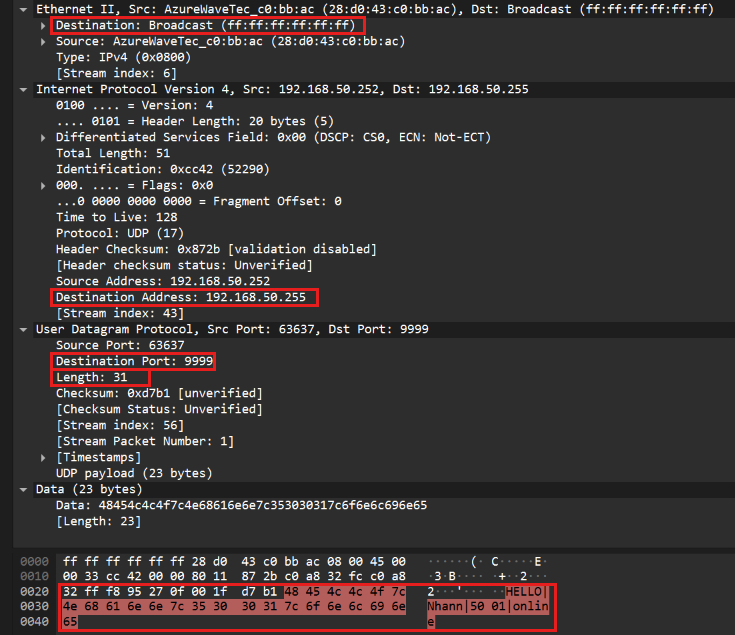
\includegraphics[width=0.85\textwidth]{wireshark_udp.png}}{\fbox{\parbox{0.9\textwidth}{\centering\vspace{2.5cm}Ảnh Wireshark gói UDP broadcast (\code{wireshark\_udp.png})\vspace{2.5cm}}}}
		\caption{Gói \code{HELLO} bắt được tại gói số 5617.}
		\label{fig:wireshark_udp}
	\end{figure}
	
	Gói số 5617 do máy Nhann phát ra:
	\begin{itemize}
		\item Địa chỉ MAC đích là \code{ff:ff:ff:ff:ff:ff} và địa chỉ IP đích là \code{192.168.50.255}, tức là broadcast của mạng \code{192.168.50.0/24}. Mọi máy trong mạng đều nhận được gói này.
		\item Cổng UDP đích là 9999, cổng nguồn là cổng ngẫu nhiên do hệ điều hành cấp.
		\item Độ dài UDP là 31 byte, gồm 8 byte tiêu đề UDP và 23 byte dữ liệu. Dữ liệu chính là chuỗi \code{HELLO|Nhann|5001|online} đã mô tả ở Mục~\ref{subsec:udp_packet}.
	\end{itemize}
	Gói của máy Long (số 7790) có cùng dạng với dữ liệu \code{HELLO|Long|5004|online}. Mỗi peer gửi lặp lại gói này mỗi 3 giây. UDP không cần bắt tay và việc mất một gói không gây hại, vì 3 giây sau gói tiếp theo sẽ được gửi.
	
	\subsection{Bắt tay ba bước của TCP}
	\begin{figure}[H]
		\centering
		\IfFileExists{wireshark_tcp.png}{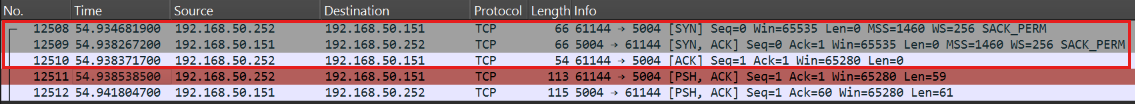
\includegraphics[width=\textwidth]{wireshark_tcp.png}}{\fbox{\parbox{0.9\textwidth}{\centering\vspace{2.5cm}Ảnh Wireshark bắt tay ba bước của TCP (\code{wireshark\_tcp.png})\vspace{2.5cm}}}}
		\caption{Bắt tay ba bước và khung \code{CHAT\_REQ}, \code{CHAT\_RESP} (gói 12508 đến 12512).}
		\label{fig:wireshark_tcp}
	\end{figure}
	
	Khi người dùng gõ \code{/chat Long}, máy Nhann mở một kết nối TCP tới máy Long (\code{192.168.50.151:5004}, cổng nguồn ngẫu nhiên 61144):
	\begin{enumerate}
		\item Gói 12508, \code{[SYN]}: máy Nhann xin mở kết nối (số thứ tự tương đối bằng 0).
		\item Gói 12509, \code{[SYN, ACK]}: máy Long đồng ý, đồng thời gửi số thứ tự của mình. Số xác nhận bằng số thứ tự của gói SYN cộng 1.
		\item Gói 12510, \code{[ACK]}: máy Nhann xác nhận. Từ đây kết nối TCP được thiết lập.
	\end{enumerate}
	Ngay sau đó, ở tầng ứng dụng, gói 12511 mang khung \code{CHAT\_REQ} do máy Nhann gửi và gói 12512 mang khung \code{CHAT\_RESP} với \code{status = accept} do máy Long trả lời, đúng như mô tả ở Mục~\ref{subsubsec:open_chat}. Wireshark hiển thị số thứ tự tương đối, nên số trong ảnh nhỏ hơn số thực tế trong gói.
	
	% ------------------------------------------------------------------------------
	% SECTION 7: KẾT LUẬN VÀ HẠN CHẾ
	% ------------------------------------------------------------------------------
	\section{Kết luận và hạn chế}
	
	\subsection{Kết quả}
	Ứng dụng đáp ứng các yêu cầu của đề tài: tự phát hiện bạn bè trong LAN, chat nhiều người, và gửi nhận tập tin có thanh tiến trình.
	
	\subsection{Hạn chế}
	\begin{itemize}
		\item Giao thức chưa có khung xác nhận (ACK). Thông báo gửi 100\% nghĩa là dữ liệu đã gửi qua socket, chưa chắc bên nhận đã lưu xong.
		\item Lời mời chat luôn được chấp nhận tự động, người nhận chưa có bước đồng ý hoặc từ chối. \code{TCPServer} đã hỗ trợ sẵn cơ chế này nhưng chưa nối vào giao diện.
		\item Dữ liệu không được mã hóa và người dùng không được xác thực. Phù hợp mạng LAN tin cậy.
		\item Việc dò các card mạng bằng lệnh \code{ipconfig} chỉ áp dụng trên Windows. Trên hệ điều hành khác chương trình dùng cách dự phòng đơn giản hơn.
	\end{itemize}
	
	\subsection{Hướng phát triển}
	Thêm khung ACK cho tin nhắn và tệp, bước đồng ý hoặc từ chối lời mời chat, mã hóa nội dung truyền, và giao diện đồ họa (nhờ phần xử lý đã tách khỏi phần giao diện, chỉ cần viết thêm một lớp giao diện mới).
	
	% ------------------------------------------------------------------------------
	% REFERENCES
	% ------------------------------------------------------------------------------
	\newpage
	\begin{thebibliography}{99}
		\bibitem{python_socket} 
		Python Software Foundation, 
		\textit{Socket --- Low-level networking interface}, Python 3 Documentation, 2026.\\
		\url{https://docs.python.org/3/library/socket.html}
		
		\bibitem{kurose_ross} 
		James F. Kurose and Keith W. Ross, 
		\textit{Computer Networking: A Top-Down Approach}, 8th Edition, Pearson, 2021.
		
		\bibitem{rfc_tcp} 
		Information Sciences Institute, University of Southern California, 
		\textit{Transmission Control Protocol (RFC 793)}, IETF, 1981.\\
		\url{https://datatracker.ietf.org/doc/html/rfc793}
		
		\bibitem{rfc_udp} 
		David P. Reed, 
		\textit{User Datagram Protocol (RFC 768)}, IETF, 1980.\\
		\url{https://datatracker.ietf.org/doc/html/rfc768}
	\end{thebibliography}
	
\end{document}